\begin{frame}
	\frametitle{第七讲、函数极限及其基本性质}
	\linespread{1.5}
	\begin{enumerate}
	  \item {\bf 内容与要求}{\color{blue}( \S3.1-3.2 )}
	  \begin{itemize}
	    \item 理解函数极限的概念
	    \item 熟练掌握函数极限的基本性质
	  \vspace{1em}
	  \end{itemize}
	  \item {\bf 课后练习:}
	  \begin{itemize}
	    \item 书面作业:{\b 习题3.1:4(1,3),6,7,10}
	    \item 思考题:{\b 习题3.1:11,12}
	  \end{itemize}
	\end{enumerate}
\end{frame}

\section{函数极限的概念}

\begin{frame}{从数列的极限出发}
	\linespread{1.6}\pause
	{\bf 数列与数列极限}\pause
	\begin{itemize}
	  \item $\{a_n\}$:\pause{\b 整序函数 $f:\mathbb{N}\to\mathbb{R}$}\pause
	  \item $\bm{\limn a_n=A}$:\pause{\b 当$n$趋于无穷时,$a_n$向确定值$A$不断逼近的趋势}\pause
 	  \item 例如:$a_n=\df 1n\to 0(n\to\infty)$
	\end{itemize}
% 	{\bf 函数与函数极限}
% 	\begin{itemize}
% 	  \item 一般函数:$f:\mathbb{R}\to\mathbb{R}$
% 	  \item \alert{$\limx{\infty} f(x)=A$}:当$x$趋于无穷时,$f(x)$向确定值$A$不断逼近的趋势
% 	\end{itemize}
\end{frame}

\begin{frame}{函数极限的六种不同趋势}
	\linespread{2}\pause
%  	{\bf 六种不同趋势}
	\begin{enumerate}
	  \item $\alert{\bm{x\to\infty\quad x\to+\infty\quad x\to -\infty}}$
	  \pause
	  \begin{itemize}
	    \item
	    $\limx{\infty}f(x)=A\Leftrightarrow\limx{+\infty}
	    f(x)=\limx{-\infty}f(x)=A$
	    \pause
	  \end{itemize}
	  \item $\alert{\bm{x\to x_0\quad x\to {x_0^+}
	  \quad x\to {x_0^-}}}$
	  \pause
	  \begin{itemize}
	    \item
	    $\limx{x_0}f(x)=A\Leftrightarrow\limx{x_0^+}f(x)=\limx{x_0^-}
	    f(x)=A$\pause
	  \end{itemize}
	\end{enumerate}
	\alert{\bf 思考:}
	{\b $\limn f(n)=A\Leftrightarrow\limx{+\infty}f(x)=A$?}\pause
	(\alert{$\times$})
\end{frame}

\begin{frame}{1、趋于无穷时的函数极限}
	\linespread{1.2}\pause 
	\begin{block}{{\bf 定义3.1.1}\hfill P103}
		\begin{enumerate}
		  \item $\bm{\limx{+\infty}f(x)=A}$\pause 
		  \begin{itemize}
		    \item $\forall\e>0,\exists X>0,\forall x>X,|f(x)-A|<\e$\pause 
		  \end{itemize}
		  \item $\bm{\limx{-\infty}f(x)=A}$\pause 
		  \begin{itemize}
		    \item $\forall\e>0,\exists X<0,\forall x<X,|f(x)-A|<\e$\pause 
		  \end{itemize}
		  \item $\bm{\limx{\infty}f(x)=A}$\pause 
		  \begin{itemize}
		    \item $\forall\e>0,\exists X>0,\forall |x|>X,|f(x)-A|<\e$
		  \end{itemize}
		\end{enumerate}
	\end{block}\pause 
	{\bf 注:}{\b $A$确定,$\e$可小,$X$可大(小),不等式可放缩}
\end{frame}

\begin{frame}{2、趋于有限值时的函数极限}
	\linespread{1.2}\pause 
	\begin{block}{{\bf 定义3.1.2}\hfill P106}
		\begin{enumerate}
		  \item $\bm{\limx{x_0}f(x)=A}$\pause 
		  \begin{itemize}
		    \item $\forall\e>0,\pause \exists \delta>0,\pause \forall
		    0<|x-x_0|<\delta,\pause |f(x)-A|<\e$\pause 
		  \end{itemize}
		  \item $\bm{\limx{x_0^+}f(x)=A}$\pause 
		  \begin{itemize}
		    \item $\forall\e>0,\exists \delta>0,\forall
		    x_0<x<x_0+\delta,|f(x)-A|<\e$\pause 
		  \end{itemize}
		  \item $\bm{\limx{x_0^-}f(x)=A}$\pause 
		  \begin{itemize}
		    \item $\forall\e>0,\exists \delta>0,\forall x_0-\delta<x<x_0,|f(x)-A|<\e$
		  \end{itemize}
		\end{enumerate}
	\end{block}\pause 
	{\bf 注:}{\b $A$确定,$\e$可小,$\delta$可小,不等式可放缩}
\end{frame}

\begin{frame}
	\linespread{1.2}
	\begin{exampleblock}{{\bf 例1:}根据图形判断极限的存在性\hfill 习题3.1-1}\pause 
		\begin{columns}
			\column{.6\textwidth}
				\begin{center}
					\resizebox{!}{3.7cm}{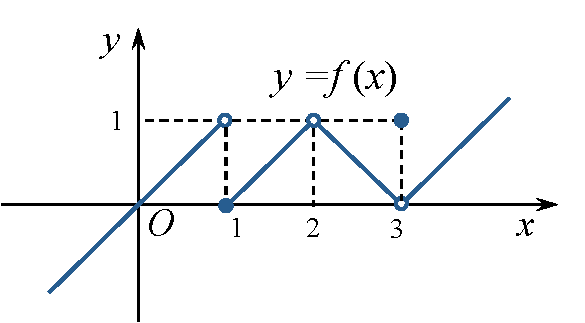
\includegraphics{./images/ch3/limxf.pdf}}
				\end{center}
			\column{.4\textwidth}
				\begin{enumerate}\pause 
				  \item $\limx{1}f(x)$\pause \underline{\alert{不存在}}\pause 
				  \item $\limx{2}f(x)$\pause \underline{\alert{\;\;$=1$\;\;\;}}\pause 
				  \item $\limx{3}f(x)$\pause \underline{\alert{\;\;$=0$\;\;\;}}\pause 
				\end{enumerate}
		\end{columns}
	\end{exampleblock}
% 	{\bf
% 	思考:}
	\begin{enumerate}
		\item {为什么在定义中要求$0<|x-x_0|<\delta$,而不是$|x-x_0|<\delta$?}\pause 
		\item {$f(x_0+0),f(x_0-0)$与$f(x_0)$是何关系?}\pause \underline{\alert{\;无关\;}}
	\end{enumerate}
\end{frame}

\begin{frame}
	\linespread{2}
	\begin{exampleblock}{{\bf 例2:}证明\hfill}
		\begin{enumerate}
		  \item $\limx{1}\df 1x=1$\pause 
% 		  \item $\limx{0^+}\df 1{\arctan x}=\df 4{\pi}$
		  \item $\limx{x_0}\sin x=\sin x_0$
		\end{enumerate}
	\end{exampleblock}
\end{frame}

\section{函数极限的基本性质}

\begin{frame}{函数极限的基本性质}
	\linespread{2}
	\begin{enumerate}\pause 
	  \item {\bf 唯一性}\pause 
	  \item {\bf 有界性}\pause 
	  \item {\bf 保号性}\pause 
	  \item {\bf 四则运算}
	\end{enumerate}
\end{frame}

\begin{frame}{唯一性}
	\linespread{1.5}\pause 
	\begin{block}{{\bf 定理3.1.2}\hfill P110}
		函数极限若存在,必唯一。
	\end{block}
\end{frame}

\begin{frame}{有界性}
	\linespread{1.5}\pause 
	\begin{block}{{\bf 定理3.1.3}\hfill P110}
		\begin{enumerate}
		  \item 若$\limx{+\infty}f(x)=A$,则$f(x)$当$x$充分大时有界\pause 
		  \item 若$\limx{x_0}f(x)=A$,则$f(x)$在$x_0$的某去心领域内有界
		\end{enumerate}
	\end{block}
\end{frame}

\begin{frame}{保号性}
	\linespread{1.5}\pause 
	\begin{block}{{\bf 定理3.1.4}\hfill P110}
		\begin{enumerate}
		  \item 若$\limx{+\infty}f(x)=A>0$,则$f(x)$当$x$充分大时大于零\pause 
		  \item 若$\limx{x_0}f(x)=A>0$,则$f(x)$在$x_0$的某去心领域内大于零
		\end{enumerate}
	\end{block}
\end{frame}

\begin{frame}{函数极限的四则运算}
	\linespread{1.5}\pause 
	\begin{block}{{\bf 定理3.2.1}\hfill P113}
		若函数极限存在,则四则运算符号可以与极限符号交换次序。
	\end{block}
\end{frame}

\begin{frame}[<+->]{小结}
	\linespread{1.5}
	\begin{enumerate}
	  \item {\bf 六种不同的趋势:}
	  \begin{itemize}
	    \item \alert{$x\to\infty,+\infty,-\infty,x_0,x_0^+,x_0^-$}
	  \end{itemize}
	  \item {\bf 极限的“$\e-\delta$”定义}
	  \begin{itemize}
	    \item \alert{$\limx{x_0}f(x)=A:\forall\e>0,\exists\delta>0,\forall
	    0<|x-x_0|<\delta,|f(x)-A|<e$}
	  \end{itemize}
	  \item {\bf 函数极限的基本性质}
	  \begin{itemize}
	    \item 唯一性、有界性、保号性、四则运算
	  \end{itemize}
	\end{enumerate}
\end{frame}

% \begin{frame}{123}
% 	\linespread{1.2}
% 	\begin{block}{{\bf 123}\hfill}
% 		123
% 	\end{block}
% \end{frame}